\documentclass[a4paper,12pt]{article}
\usepackage{epsfig,latexsym,amsmath,amssymb,epic,eepic,psfrag,subfigure,float,euscript,array}
\usepackage[latin1]{inputenc}
\usepackage{standalone}
\usepackage{tikz,pgf,pgfplots}

\newenvironment{exercise}[1][Uppgift]{\begin{trivlist} \item[\hskip
    \labelsep {\stepcounter{exerctr}\bfseries #1
      \arabic{exerctr}}]}{\end{trivlist}\vspace{10mm}}

\newcounter{exerctr}
\newcounter{abcctr}[exerctr]

\newcommand{\abc}{\noindent\vspace{1mm}\\ {\bf
    \stepcounter{abcctr}(\alph{abcctr})\ }}
\newcommand{\bbm}{\begin{bmatrix}}
\newcommand{\ebm}{\end{bmatrix}}
\newcommand{\point}[1]{\hfill {\bf (#1p)}\\ \vspace{-5mm}}
\newcommand{\ctrb}{\EuScript{S}}
\newcommand{\Lap}{\mathcal{L}}
\newcommand{\obsv}{\EuScript{O}}
\newcommand{\realdel}[1]{\text{Re}\left\{#1\right\}}
\newcommand{\imagdel}{\text{Im}}
\newcommand{\bC}{\mathbb{C}}
\newcommand{\bR}{\mathbb{R}}
\newcommand{\bmpv}{\begin{minipage}[t]}
\newcommand{\bmps}{\begin{minipage}[t]{45mm}}
\newcommand{\bmpm}{\begin{minipage}[t]{90mm}}
\newcommand{\bmpl}{\begin{minipage}[t]{140mm}}
\newcommand{\emp}{\end{minipage}}
\newcommand*{\zethree}{\big(z - \mexp{-3h}\big)}
\newcommand*{\mexp}[1]{\ensuremath{\mathrm{e}^{#1}}}

\addtolength{\topmargin}{-1cm}
\textheight 23.5cm
%\oddsidemargin 0.61cm
%\evensidemargin 0.61cm


\def\OctaveG{tf([0.5 1], [1 0 -1])}

\title{Computerized control partial exam 1 (15\%)}
\author{Kjartan Halvorsen}

\begin{document}

\maketitle


\begin{description}
\item[Time] September 13 17:30
\item[Place] 4101
\item[Permitted aids] The single colored page with your own notes, table of Laplace transforms, calculator
\end{description}

All answers should be readable and well motivated (if nothing else is written). Solutions/motivations should be written on the provided spaces in this exam. Use the last page if more space is needed.

\begin{center}
{\Large Good luck!} \\
\end{center}

\begin{tabular}{|l|l|}
\hline
\multicolumn{2}{|l|}{\bmpl
Matricula and name
\vspace*{18mm}
\emp}\\
\hline

\end{tabular}

\clearpage

%-----------------------------------------------------------------
\subsection*{The system}
The dynamic model of a ship with input $u$ being the rudder angle and the output $y$ being the heading (see figure \ref{fig:tanker}) can be described as a continuous-time second order system with a pole in the origin
\[ G(s) = \frac{K}{s(s + a)}. \]
For fully loaded, large tankers this dynamics is often unstable, meaning that $a<0$.  
\begin{figure}[h]
\begin{center}
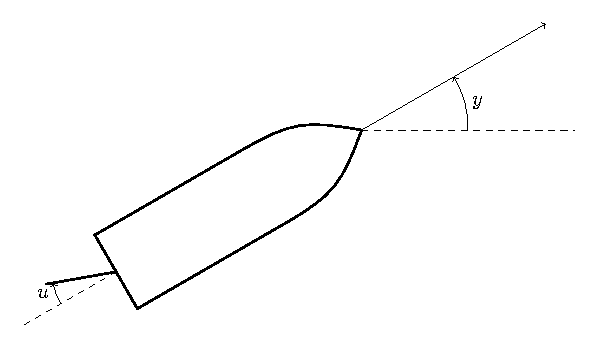
\includegraphics[width=0.8\linewidth]{tanker}
\caption{Heading of a ship controlled by rudder input.}
\label{fig:tanker}
\end{center}
\end{figure}

Consider for this exam the normalized continuous-time model of the tanker
\[ G(s) = \frac{1}{s(s - 1)}. \]

\clearpage
\subsection*{Problem 1 (50p)}

The system is sampled with sampling interval $h$ using step-invariant (zero-order hold) sampling. \textbf{Circle the correct pulse-transfer function below, and show your calculations}
\begin{enumerate}
 \item \( H(z) = \frac{(1-\mexp{h} -h)z - \big((1-h)\mexp{h}-1\big)}{(z-1)(z-\mexp{h})}\)
 \item \( H(z) = \frac{(-1+\mexp{h} -h)z - \big((1-h)\mexp{h}-1\big)}{(z-1)(z-\mexp{2h})}\)
 \item \( H(z) = \frac{(-1+\mexp{h} -h)z - \big((1-h)\mexp{h}-1\big)}{(z-1)(z-\mexp{h})}\)
 \end{enumerate}

\noindent
\fbox{
\bmpl
{\bf Derivation:}\\
\vspace*{150mm}
\emp}

\clearpage
\subsection*{Problem 2 (20p)}
Assume that the sampling period is $h=0.2$. In figure \ref{fig:complex-plane} draw the poles (crosses) and zero (circle) for both the continuous-time transfer function $G(s)$ and the  discretized pulse-transfer function $H(z)$ you determined in Problem 1.
   \begin{figure}[h]
   \begin{center}
   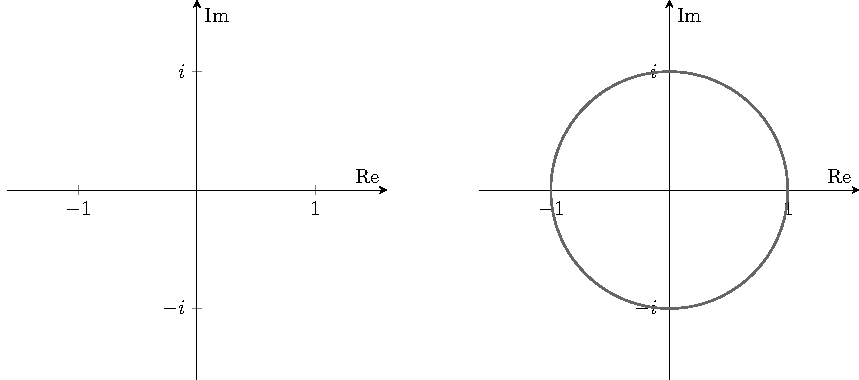
\includegraphics[]{complex-plane}
   \caption{Problem 2: Plot the poles of the continuous-time system (on the left) and the poles and zero of the discrete-time system (on the right). Indicate (with arrows and/or colors) corresponding pairs of continuous-time and discrete-time poles.}
   \label{fig:complex-plane}
   \end{center}
   \end{figure}

\noindent
\fbox{
\bmpl
{\bf Calculations:}\\
\vspace*{90mm}
\emp}

\clearpage

\subsection*{Problem 3 (30p)}
The tanker is stabilized using error-feedback and a lead-compensator as in the figure below. 
\begin{center}
  \includestandalone[width=0.5\linewidth]{feedback-lead}
\end{center}
The design is done in continuous-time giving the controller
\[ F(s) = 20 \frac{s+1}{s+6}. \]
Suggest a discretization method (give short motivation) and discretize the controller. Write the controller as a first order difference equation

\noindent
\fbox{
\bmpl
{\bf Solutions:}\\
\vspace*{140mm}
\emp}

\clearpage

\noindent
{\bf If necessary,} you can continue your solutions on this page. Mark clearly which problem the solution corresponds to.


%\end{document}

%*****************************************************************
%*****************************************************************
\newpage
\setcounter{page}{1}

\section*{Solutions}
\subsection*{Problem 1}
   First calculate the step-response of the continous-time system
   \[Y(s) = G(s)\frac{1}{s} = \frac{1}{s^2(s-1)} = \frac{1}{s-1} - \frac{1}{s} - \frac{1}{s^2}.\]
   The inverse Laplace-transform gives
   \[ y(t) = \mexp{t} - 1 - t\]
   Sampling this function gives
   \[ y(kh) = \mexp{kh} -1 - kh\]
   which has the Z-transform
   \[Y(z) = \frac{z}{z - \mexp{h}} - \frac{z}{z-1} - \frac{hz}{(z-1)^2}\]
   Dividing the z-transform of the system response to that of the input (the step) gives
   \begin{align*}
   H(z) &= \frac{Y(z)}{U(z)} = \frac{z-1}{z}Y(z) = \frac{z-1}{z-\mexp{h}} - 1 - \frac{h}{z-1}\\
        &= \frac{(z-1)^2 - (z-1)(z-\mexp{h}) - h(z-\mexp{h})}{(z-1)(z-\mexp{h})}\\
	&= \frac{(z-1)(z-1 -z + \mexp{h}) - hz + h\mexp{h}}{(z-1)(z-\mexp{h})}\\
        &= \frac{ (\mexp{h} - 1 -h)z - (\mexp{h}-1-h\mexp{h})}{(z-1)(z-\mexp{h})}\\
        &= \frac{ (\mexp{h} - 1 -h)z - \big( (1-h)\mexp{h}-1\big)}{(z-1)(z-\mexp{h})}\\
   \end{align*}

   The correct pulse transfer function is the third.

\subsection*{Problem 2}
The discrete-time poles are in $z=1$ and $z=\mexp{0.2} \approx 1.22$. The zero is  in 
\[ z = - \frac{(1-h)\mexp{0.2} - 1}{\mexp{0.2} - 1 -h} \approx -1.07. \]
\begin{center}
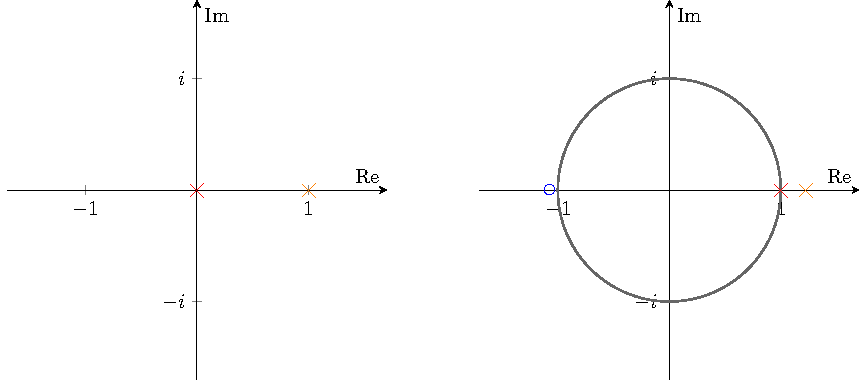
\includegraphics[width=0.8\linewidth]{complex-plane-facit}
\end{center}
 
\subsection*{Problem 3}
Tustin's approximation should give reasonable performance, since it is a better approximation than backward or forward difference. It is also easy to apply. The approximation gives the pulse-transfer function
\[ F_d(z) = F(s)|_{s= \frac{2(z-1)}{h(z+1)}} = 20 \frac{ \frac{2(z-1)}{h(z+1)} + 1 }{ \frac{2(z-1)}{h(z+1)} + 6} = 20 \frac{2(z-1) + h(z+1)}{2(z-1) + 6h(z+1)} = 20 \frac{(2+h)z - (2-h)}{(2+6h)z - (2-6h)} \]
We get
\[ U(z) = F_d(z)E(z) = 20 \frac{(2+h)z - (2-h)}{(2+6h)z - (2-6h)} E(z) \]
or
\[ \big( (2+6h) z - (2-6h) \big) U(z) = 20 \big( (2+h)z - (2-h) \big) E(z). \]
Written as a difference equation 
\[ (2+6h) u(kh+h) - (2-6h)u(kh) = 20 (2+h) e(kh+h) - 20 (2-h) e(kh)\]
or
\[ u(kh+h) = \frac{2-6h}{2+6h} u(kh) + \frac{20(2+h)}{2+6h} e(kh+h) - \frac{20(2-h)}{2+6h} e(kh). \]

\end{document}
